\begin{figure}[ht]
    \begin{tabularx}{\linewidth}{Y Y}
        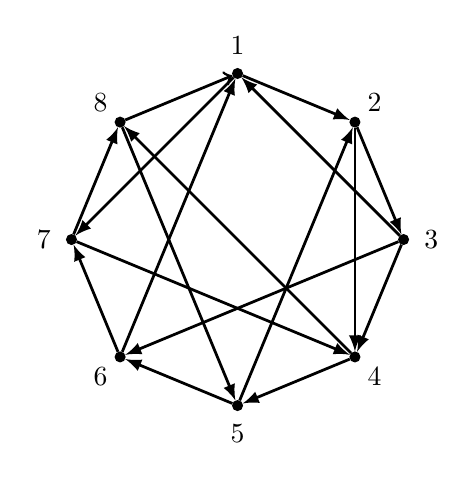
\begin{tikzpicture}
            \foreach \angle [count = \xi] in {90, 45, ..., -235}
                {
                    \node[circle, fill, minimum size=.4em, inner sep=0pt, outer sep=0pt] (node\xi) at (\angle:6em) {};
                    \node (nodetext\xi) at (\angle:7em) {\xi};
                }
            \foreach \xi in {2, 3, ..., 8}
                {
                    \pgfmathtruncatemacro\xii{\xi - 1};
                    \draw[-latex,line width = .1em] (node\xii) -- (node\xi);
                }
            \draw[->,line width = .1em] (node8) -- (node1);
            \foreach \x/\y in {3/1, 5/2, 2/4, 3/6, 8/5, 1/7, 7/4, 6/1, 4/8}
                {
                    \draw[-latex, line width = .1em] (node\x) -- (node\y);
                }
        \end{tikzpicture}
         &
        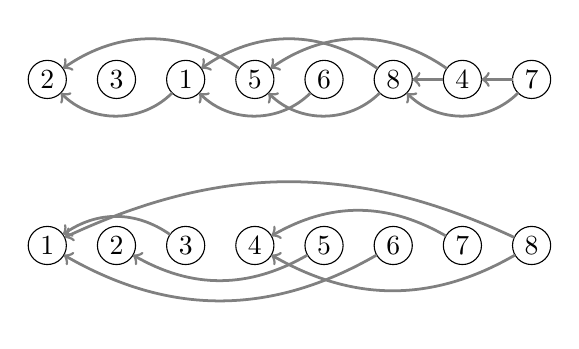
\begin{tikzpicture}
            \node[circle, fill = white, draw = black, inner sep = .2em, outer sep=0pt] (node2) {2};
            \foreach \xi [count = \xii] in {3, 1, 5, 6, 8, 4, 7}
                {
                    \pgfmathsetmacro\dist{\xii * 2.5};
                    \node[circle, fill = white, draw = black, inner sep = .2em, outer sep=0pt] at ([xshift = \dist em]node2)(node\xi) {\xi};
                }
            \draw[bend right = 35, ->, line width = .1em, gray]  (node5) to node [auto] {} (node2);
            \draw[bend left = 45, ->, line width = .1em, gray]  (node8) to node [auto] {} (node5);
            \draw[->, line width = .1em, gray] (node7) -- (node4);
            \draw[->, line width = .1em, gray] (node4) -- (node8);
            \draw[bend left = 45, ->, line width = .1em, gray]  (node6) to node [auto] {} (node1);
            \draw[bend left = 45, ->, line width = .1em, gray]  (node1) to node [auto] {} (node2);
            \draw[bend right = 35, ->, line width = .1em, gray]  (node4) to node [auto] {} (node5);
            \draw[bend left = 45, ->, line width = .1em, gray]  (node7) to node [auto] {} (node8);
            \draw[bend right = 35, ->, line width = .1em, gray]  (node8) to node [auto] {} (node1);

            \node[circle, fill = white, draw = black, inner sep = .2em, outer sep=0pt] at ([yshift = -6em]node2) (node21) {1};
            \foreach \xi [count = \xii] in {2, 3, ..., 8}
                {
                    \pgfmathsetmacro\dist{\xii * 2.5};
                    \node[circle, fill = white, draw = black, inner sep = .2em, outer sep=0pt] at ([xshift = \dist em]node21)(node2\xi) {\xi};
                }

            \draw[bend left = 30, ->, line width = .1em, gray]  (node25) to node [auto] {} (node22);
            \draw[bend right = 35, ->, line width = .1em, gray]  (node23) to node [auto] {} (node21);
            \draw[bend left = 30, ->, line width = .1em, gray]  (node26) to node [auto] {} (node21);
            \draw[bend right = 30, ->, line width = .1em, gray]  (node27) to node [auto] {} (node24);
            \draw[bend right = 25, ->, line width = .1em, gray]  (node28) to node [auto] {} (node21);
            \draw[bend left = 30, ->, line width = .1em, gray]  (node28) to node [auto] {} (node24);
        \end{tikzpicture}
        \\
        (a) dependency graph $G_{\profileSet, \varphi}$ \linebreak
         &
        (b) $(\varphi, \DBW)$-fair-order (above) and lexicographic order (below)
        \\
    \end{tabularx}
    \addtocounter{table}{-1}
    \medskip

    \caption{Illustration of a dependency graph, a $(\varphi, \DBW)$-fair-order and a lexicographic order on \profileSet. Only back edges are illustrated in (b).}
    \label{fig:optimal-bandwidth-order}
\end{figure}